\documentclass[11pt,letterpaper]{article}
\usepackage[margin=0.75in]{geometry}
\usepackage{amsmath}
\usepackage{tikz}
\usepackage{hyperref}
\usetikzlibrary{patterns,decorations.pathreplacing,calc,arrows.meta}

\title{\textbf{Chapter 5: LEO Coverage} \\ Visual Guide with Diagrams}
\author{SPCE 5400 - Ground Station Design}
\date{}

\begin{document}

\maketitle

\section*{Figure 5.2: LEO Coverage Area Geometry}

This is the most critical diagram showing the geometric relationships for coverage calculations.

\begin{center}
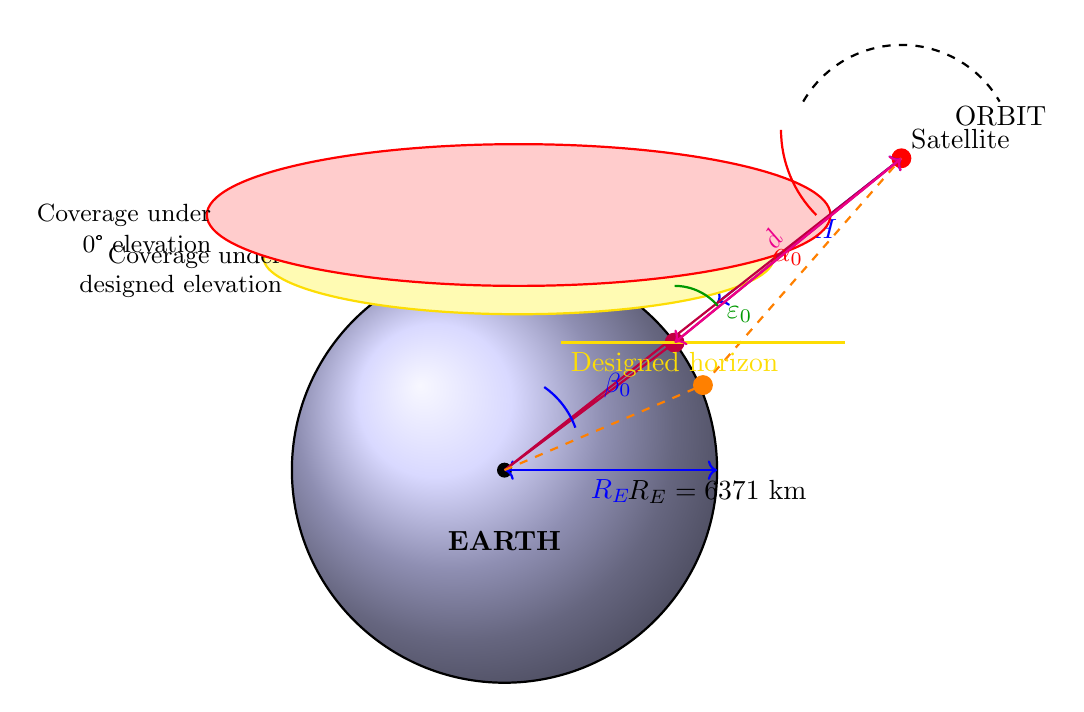
\begin{tikzpicture}[scale=1.8]
    % Earth
    \shade[ball color=blue!20] (0,0) circle (1.5cm);
    \draw[thick] (0,0) circle (1.5cm);
    \node at (0,-0.5) {\textbf{EARTH}};

    % Earth center
    \fill (0,0) circle (1.5pt);

    % Satellite at altitude H
    \coordinate (sat) at (2.8,2.2);
    \fill[red] (sat) circle (2pt);
    \node[above right] at (sat) {Satellite};

    % Ground station on designed horizon
    \coordinate (gs_designed) at (1.2,0.9);
    \fill[purple] (gs_designed) circle (2pt);

    % Ground station on ideal horizon
    \coordinate (gs_ideal) at (1.4,0.6);
    \fill[orange] (gs_ideal) circle (2pt);

    % Altitude line
    \draw[dashed] (0,0) -- (sat);
    \draw[<->,thick,blue] (0,0) -- (1.5,0);
    \node[below,blue] at (0.75,0) {$R_E$};

    \draw[<->,thick,blue] (1.5,1.18) -- (sat);
    \node[right,blue] at (2.1,1.7) {$H$};

    % Orbit path
    \draw[thick,dashed] (sat) ++ (150:0.8) arc (150:30:0.8);
    \node at (3.5,2.5) {ORBIT};

    % Coverage under designed elevation (smaller yellow circle)
    \draw[thick,yellow!80!orange,fill=yellow!30] (0.1,1.5) ellipse (1.8cm and 0.4cm);
    \node[left] at (-1.5,1.5) {\small Coverage under};
    \node[left] at (-1.5,1.3) {\small designed elevation};

    % Coverage under 0° elevation (larger red circle)
    \draw[thick,red,fill=red!20] (0.1,1.8) ellipse (2.2cm and 0.5cm);
    \node[left] at (-2.0,1.8) {\small Coverage under};
    \node[left] at (-2.0,1.6) {\small 0° elevation};

    % Triangle for designed elevation
    \draw[thick,purple] (0,0) -- (gs_designed) -- (sat) -- cycle;

    % Triangle for ideal elevation
    \draw[thick,orange,dashed] (0,0) -- (gs_ideal) -- (sat);

    % Angles
    % Nadir angle alpha_0
    \draw[thick,red] (2.2,1.8) arc (225:180:0.85);
    \node[red] at (2.0,1.5) {$\alpha_0$};

    % Elevation angle epsilon_0
    \draw[thick,green!60!black] (gs_designed) ++ (40:0.4) arc (40:90:0.4);
    \node[green!60!black,right] at (1.5,1.1) {$\varepsilon_0$};

    % Central angle beta_0
    \draw[thick,blue] (0.5,0.3) arc (20:55:0.6);
    \node[blue] at (0.8,0.6) {$\beta_0$};

    % Designed horizon plane
    \draw[thick,yellow!80!orange] (gs_designed) -- ++ (180:0.8);
    \draw[thick,yellow!80!orange] (gs_designed) -- ++ (0:1.2);
    \node[below,yellow!80!orange] at (gs_designed) {Designed horizon};

    % Slant range d
    \draw[<->,thick,magenta] (gs_designed) -- (sat);
    \node[magenta,above,rotate=55] at (2.0,1.55) {$d$};

    % Labels
    \node[below] at (1.5,0) {$R_E = 6371$ km};

\end{tikzpicture}
\end{center}

\textbf{Key Relationships:}
\begin{itemize}
    \item $\varepsilon_0 + \alpha_0 + \beta_0 = 90°$
    \item $\sin \alpha_0 = \frac{R_E}{R_E + H} \cos \varepsilon_0$
    \item $C[\%] = \frac{1}{2}(1 - \cos\beta_0)$
\end{itemize}

\newpage

\section*{Figure 5.5: Virtual Coverage Movement}

Shows how coverage area moves as satellite orbits while Earth rotates.

\begin{center}
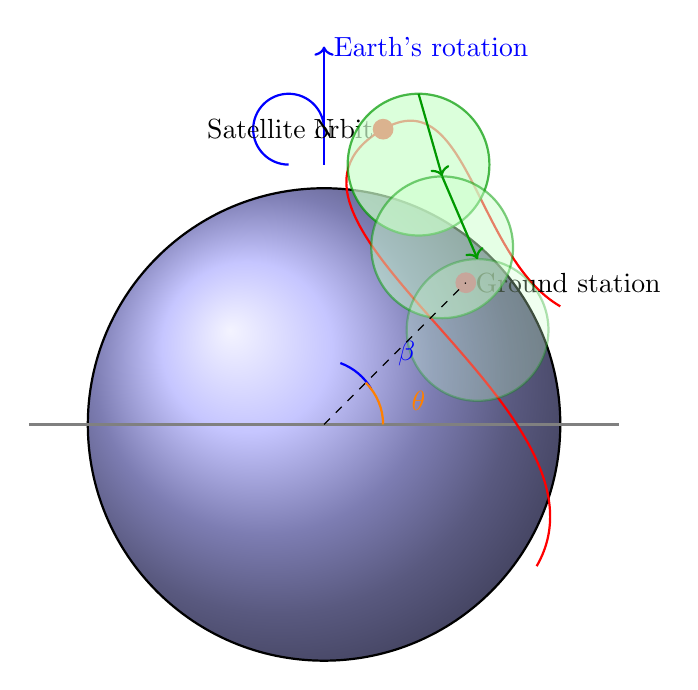
\begin{tikzpicture}[scale=1.5]
    % Earth
    \shade[ball color=blue!30] (0,0) circle (2cm);
    \draw[thick] (0,0) circle (2cm);

    % Equator
    \draw[thick,gray] (-2.5,0) -- (2.5,0);

    % Earth rotation axis
    \draw[thick,blue,->] (0,2.2) -- (0,3.2);
    \node[right,blue] at (0,3.2) {Earth's rotation};
    \draw[thick,blue] (0,2.5) arc (0:270:0.3);

    % North pole
    \node at (0,2.5) {N};

    % Satellite orbit (inclined)
    \draw[thick,red] (1.8,-1.2) to[out=60,in=210] (0.5,2.5) to[out=30,in=150] (2,1);
    \fill[red] (0.5,2.5) circle (2.5pt);
    \node[left] at (0.5,2.5) {Satellite orbit};

    % Ground station
    \fill[purple] (1.2,1.2) circle (2.5pt);
    \node[right] at (1.2,1.2) {Ground station};

    % Coverage footprint at different positions
    \draw[thick,green!60!black,fill=green!20,opacity=0.7] (0.8,2.2) circle (0.6cm);
    \draw[thick,green!60!black,fill=green!20,opacity=0.5] (1.0,1.5) circle (0.6cm);
    \draw[thick,green!60!black,fill=green!20,opacity=0.3] (1.3,0.8) circle (0.6cm);

    % Arrows showing movement
    \draw[->,thick,green!60!black] (0.8,2.8) -- (1.0,2.1);
    \draw[->,thick,green!60!black] (1.0,2.1) -- (1.3,1.4);

    % Central angle beta
    \draw[thick,blue] (0.4,0.3) arc (30:70:0.5);
    \node[blue] at (0.7,0.6) {$\beta$};

    % Theta angle
    \draw[dashed] (0,0) -- (1.2,1.2);
    \draw[thick,orange] (0.5,0) arc (0:45:0.5);
    \node[orange] at (0.8,0.2) {$\theta$};

\end{tikzpicture}
\end{center}

\textbf{Key Concepts:}
\begin{itemize}
    \item Coverage footprint moves vertically along satellite's orbital path
    \item Earth rotates horizontally (eastward) around N-S axis
    \item Coverage belt moves westward relative to Earth's rotation
    \item Single satellite provides global access but not simultaneously
\end{itemize}

\newpage

\section*{Figure 5.6: Coverage Belt}

The area swept by satellite's coverage during one complete orbit.

\begin{center}
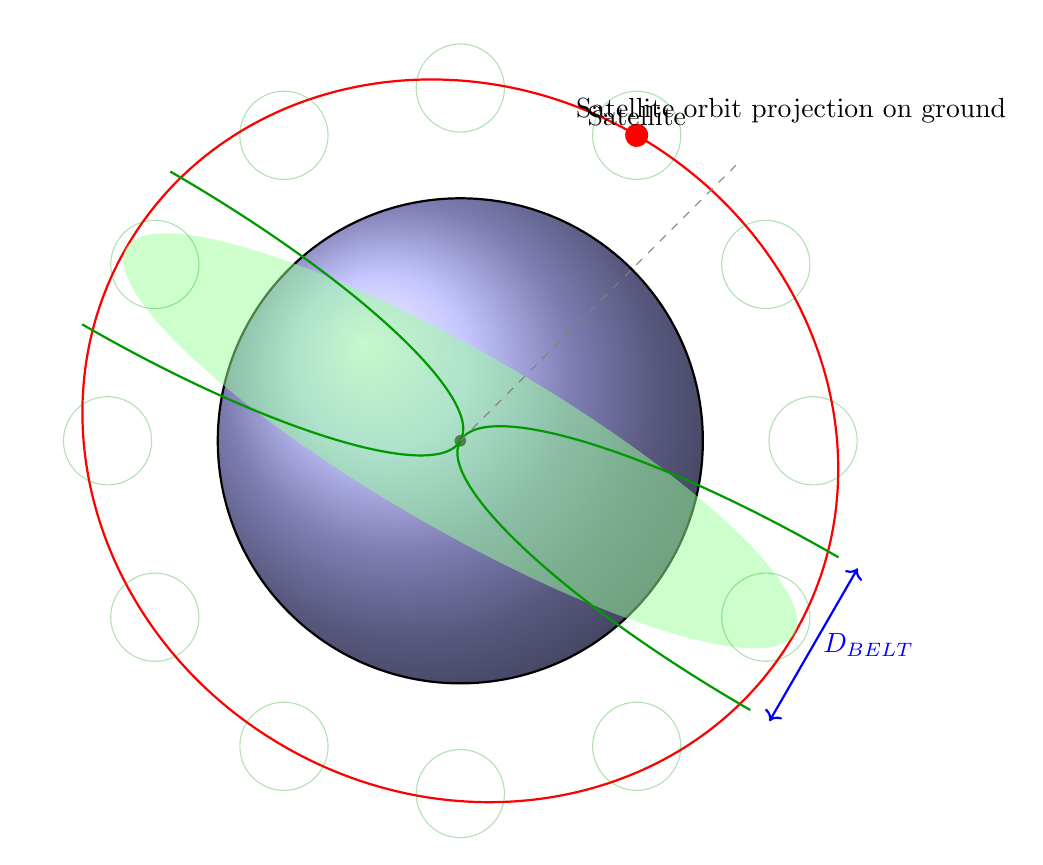
\begin{tikzpicture}[scale=1.4]
    % Earth
    \shade[ball color=blue!30] (0,0) circle (2.2cm);
    \draw[thick] (0,0) circle (2.2cm);

    % Earth center
    \fill (0,0) circle (1.5pt);

    % Satellite orbit
    \begin{scope}[rotate=-30]
        \draw[thick,red] (0,0) ellipse (3.5cm and 3.2cm);

        % Coverage belt (shaded region)
        \fill[green!40,opacity=0.5] (0,0) ellipse (3.5cm and 0.8cm);
        \draw[thick,green!60!black] (3.5,0.8) arc (90:270:3.5cm and 0.8cm);
        \draw[thick,green!60!black] (-3.5,0.8) arc (90:-90:3.5cm and 0.8cm);

        % Belt width arrows
        \draw[<->,thick,blue] (3.7,0.8) -- (3.7,-0.8);
        \node[right,blue] at (3.7,0) {$D_{BELT}$};

        % Satellite at orbit
        \fill[red] (0,3.2) circle (3pt);
        \node[above] at (0,3.2) {Satellite};

        % Coverage circles along orbit
        \foreach \angle in {0,30,60,...,330} {
            \draw[green!60!black,opacity=0.3] (\angle:3.2) circle (0.4cm);
        }
    \end{scope}

    % Projection lines
    \draw[dashed,gray] (0,0) -- (2.5,2.5);
    \node at (3,3) {Satellite orbit projection on ground};

\end{tikzpicture}
\end{center}

\textbf{Coverage Belt Width:}
\begin{align*}
D_{BELT} &= 2d_{max} \\
d_{max} &= R_E \left[\sqrt{\left(\frac{H + R_E}{R_E}\right)^2 - 1}\right]
\end{align*}

\textbf{Key Points:}
\begin{itemize}
    \item Belt width depends on altitude $H$ and elevation angle $\varepsilon_0$
    \item Wider at higher altitudes
    \item Narrower at higher elevation angles
    \item Range: 3857 to 8178 km for typical LEO altitudes
\end{itemize}

\newpage

\section*{Figure 5.8: Coverage Belt of Different Satellite Altitudes}

Comparison showing how altitude affects coverage belt width.

\begin{center}
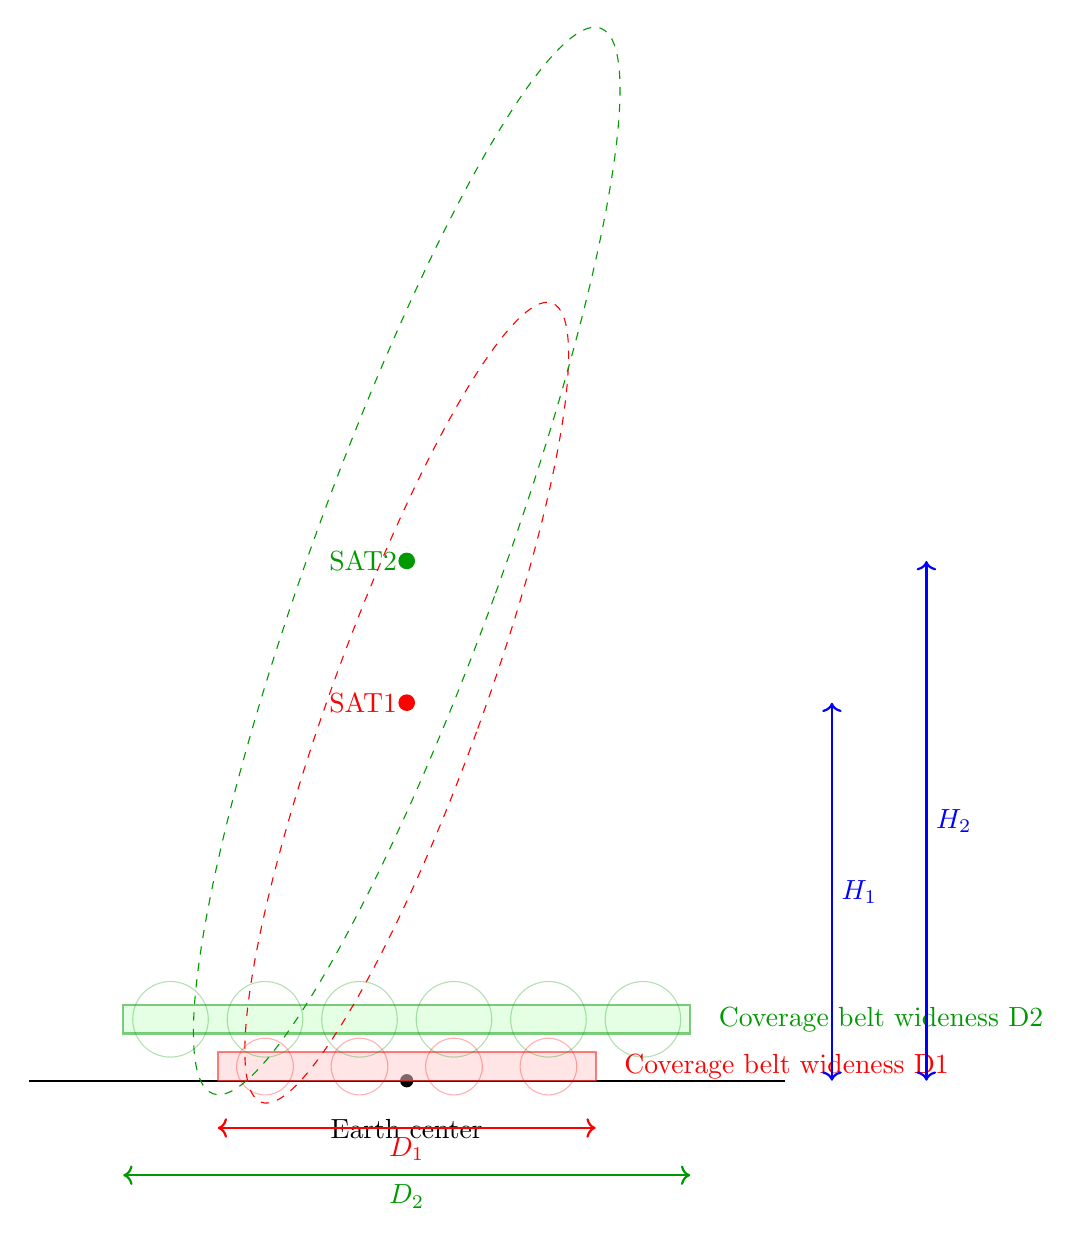
\begin{tikzpicture}[scale=1.2]
    % Earth center reference
    \fill (0,0) circle (2pt);
    \node[below] at (0,-0.3) {Earth center};

    % Satellite 1 at lower altitude (H1)
    \coordinate (sat1) at (0,4);
    \fill[red] (sat1) circle (2.5pt);
    \node[left,red] at (sat1) {SAT1};

    % Satellite 2 at higher altitude (H2)
    \coordinate (sat2) at (0,5.5);
    \fill[green!60!black] (sat2) circle (2.5pt);
    \node[left,green!60!black] at (sat2) {SAT2};

    % Earth surface (simplified as horizontal line)
    \draw[thick] (-4,0) -- (4,0);

    % Coverage belt for SAT1 (narrower)
    \draw[thick,red,fill=red!20,opacity=0.5] (-2,0) -- (-2,0.3) -- (2,0.3) -- (2,0) -- cycle;
    \draw[<->,thick,red] (-2,-0.5) -- (2,-0.5);
    \node[below,red] at (0,-0.5) {$D_1$};
    \node[red,right] at (2.2,0.15) {Coverage belt wideness D1};

    % Coverage belt for SAT2 (wider)
    \draw[thick,green!60!black,fill=green!20,opacity=0.5] (-3,0.5) -- (-3,0.8) -- (3,0.8) -- (3,0.5) -- cycle;
    \draw[<->,thick,green!60!black] (-3,-1.0) -- (3,-1.0);
    \node[below,green!60!black] at (0,-1.0) {$D_2$};
    \node[green!60!black,right] at (3.2,0.65) {Coverage belt wideness D2};

    % Altitudes
    \draw[<->,thick,blue] (4.5,0) -- (4.5,4);
    \node[right,blue] at (4.5,2) {$H_1$};

    \draw[<->,thick,blue] (5.5,0) -- (5.5,5.5);
    \node[right,blue] at (5.5,2.75) {$H_2$};

    % Orbit projections
    \begin{scope}[rotate=-20]
        \draw[dashed,red] (sat1) ellipse (0.8cm and 4.5cm);
        \draw[dashed,green!60!black] (sat2) ellipse (1.0cm and 6.0cm);
    \end{scope}

    % Coverage circles
    \foreach \x in {-1.5,-0.5,0.5,1.5} {
        \draw[red,opacity=0.3] (\x,0.15) circle (0.3cm);
    }

    \foreach \x in {-2.5,-1.5,-0.5,0.5,1.5,2.5} {
        \draw[green!60!black,opacity=0.3] (\x,0.65) circle (0.4cm);
    }

\end{tikzpicture}
\end{center}

\textbf{Relationship:}
\begin{itemize}
    \item Higher altitude ($H_2 > H_1$) → Wider coverage belt ($D_2 > D_1$)
    \item SAT2 at 1200 km: $D_{BELT}$ = 8177.8 km (at $\varepsilon_0 = 0°$)
    \item SAT1 at 600 km: $D_{BELT}$ = 5633.0 km (at $\varepsilon_0 = 0°$)
\end{itemize}

\newpage

\section*{Figure 5.9: Coverage Belt Variation Graph}

Shows how coverage belt width varies with elevation angle for different altitudes.

\begin{center}
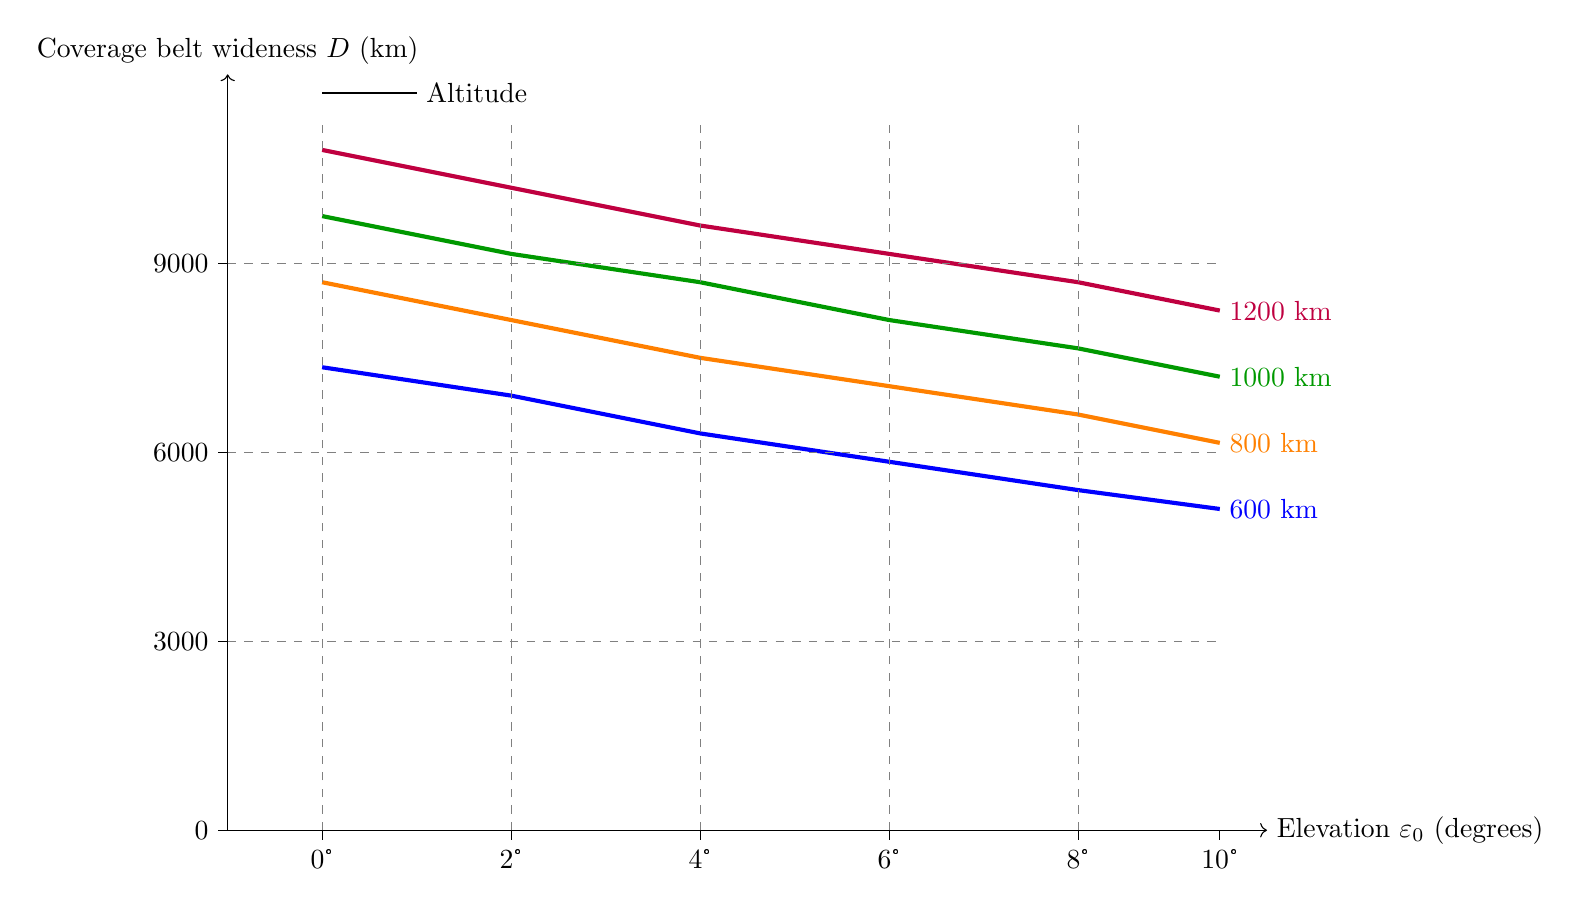
\begin{tikzpicture}[scale=1.2]
    % Axes
    \draw[->] (0,0) -- (11,0) node[right] {Elevation $\varepsilon_0$ (degrees)};
    \draw[->] (0,0) -- (0,8) node[above] {Coverage belt wideness $D$ (km)};

    % Y-axis labels
    \foreach \y/\label in {0/0, 2/3000, 4/6000, 6/9000} {
        \draw (0,\y) -- (-0.1,\y) node[left] {\label};
    }

    % X-axis labels (elevation angles)
    \foreach \x/\label in {1/0, 3/2, 5/4, 7/6, 9/8, 10.5/10} {
        \draw (\x,0) -- (\x,-0.1) node[below] {\label°};
    }

    % Data curves (approximate from Table 5.2)
    % 1200 km (top curve - purple)
    \draw[thick,purple,line width=1.5pt]
        (1,7.2) -- (3,6.8) -- (5,6.4) -- (7,6.1) -- (9,5.8) -- (10.5,5.5);
    \node[purple,right] at (10.5,5.5) {1200 km};

    % 1000 km (green)
    \draw[thick,green!60!black,line width=1.5pt]
        (1,6.5) -- (3,6.1) -- (5,5.8) -- (7,5.4) -- (9,5.1) -- (10.5,4.8);
    \node[green!60!black,right] at (10.5,4.8) {1000 km};

    % 800 km (orange)
    \draw[thick,orange,line width=1.5pt]
        (1,5.8) -- (3,5.4) -- (5,5.0) -- (7,4.7) -- (9,4.4) -- (10.5,4.1);
    \node[orange,right] at (10.5,4.1) {800 km};

    % 600 km (bottom curve - blue)
    \draw[thick,blue,line width=1.5pt]
        (1,4.9) -- (3,4.6) -- (5,4.2) -- (7,3.9) -- (9,3.6) -- (10.5,3.4);
    \node[blue,right] at (10.5,3.4) {600 km};

    % Legend
    \draw[thick] (1,7.8) -- (2,7.8);
    \node[right] at (2,7.8) {Altitude};

    % Grid (light)
    \foreach \x in {1,3,5,7,9} {
        \draw[gray,very thin,dashed] (\x,0) -- (\x,7.5);
    }
    \foreach \y in {2,4,6} {
        \draw[gray,very thin,dashed] (0,\y) -- (10.5,\y);
    }

\end{tikzpicture}
\end{center}

\textbf{Key Observations:}
\begin{enumerate}
    \item All curves decrease as elevation increases (narrower belt at higher elevation)
    \item Higher altitude curves are above lower altitude curves (wider belts)
    \item Steepest decrease occurs at low elevations (0-4°)
    \item At 10° elevation, belt widths range from 3857 km (600km) to 6274 km (1200km)
\end{enumerate}

\newpage

\section*{Figure 5.12: LEO Overlapped Coverage Area}

Constellation with overlapping coverage zones for handover.

\begin{center}
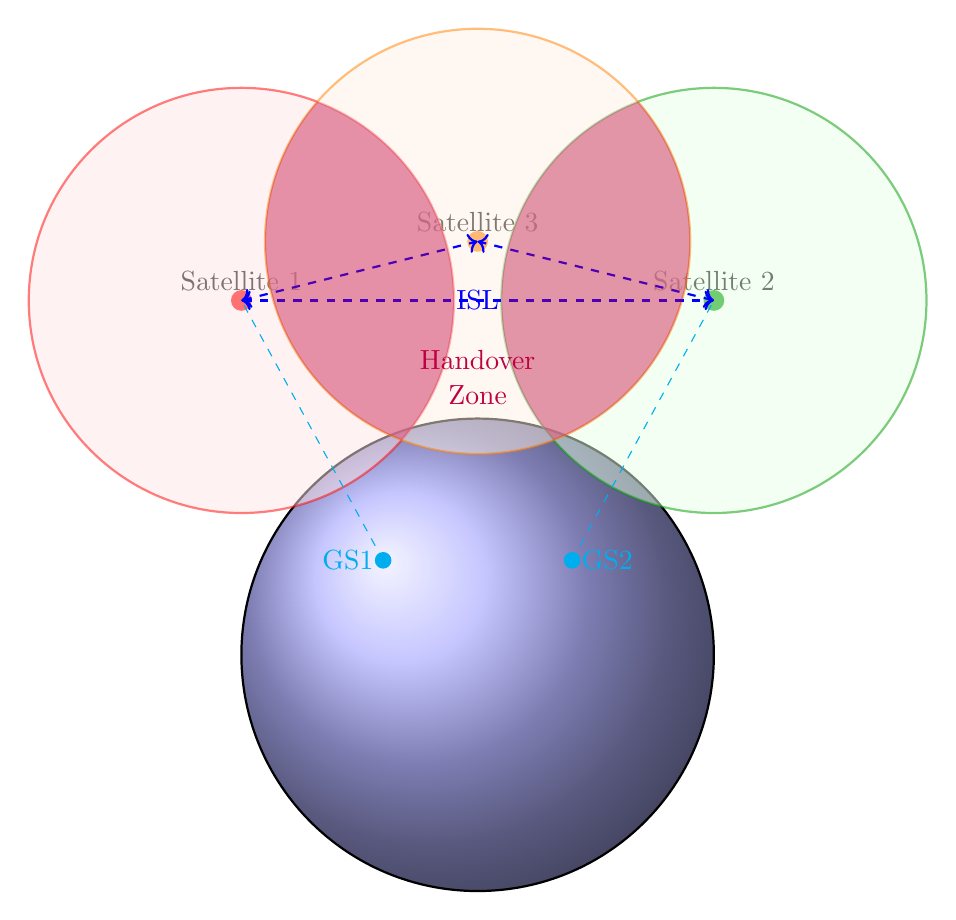
\begin{tikzpicture}[scale=1.5]
    % Earth
    \shade[ball color=blue!30] (0,0) circle (2cm);
    \draw[thick] (0,0) circle (2cm);

    % Satellite 1
    \coordinate (sat1) at (-2,3);
    \fill[red] (sat1) circle (2.5pt);
    \node[above] at (sat1) {Satellite 1};

    % Satellite 2
    \coordinate (sat2) at (2,3);
    \fill[green!60!black] (sat2) circle (2.5pt);
    \node[above] at (sat2) {Satellite 2};

    % Satellite 3
    \coordinate (sat3) at (0,3.5);
    \fill[orange] (sat3) circle (2.5pt);
    \node[above] at (sat3) {Satellite 3};

    % Coverage circles
    \draw[thick,red,fill=red!10,opacity=0.5] (sat1) circle (1.8cm);
    \draw[thick,green!60!black,fill=green!10,opacity=0.5] (sat2) circle (1.8cm);
    \draw[thick,orange,fill=orange!10,opacity=0.5] (sat3) circle (1.8cm);

    % Intersatellite links
    \draw[thick,blue,dashed,<->] (sat1) -- (sat2);
    \draw[thick,blue,dashed,<->] (sat1) -- (sat3);
    \draw[thick,blue,dashed,<->] (sat2) -- (sat3);
    \node[blue] at (0,3) {ISL};

    % Overlap zones (darker shaded)
    \begin{scope}
        \clip (sat1) circle (1.8cm);
        \fill[purple,opacity=0.4] (sat2) circle (1.8cm);
    \end{scope}

    \begin{scope}
        \clip (sat2) circle (1.8cm);
        \fill[purple,opacity=0.4] (sat3) circle (1.8cm);
    \end{scope}

    \begin{scope}
        \clip (sat1) circle (1.8cm);
        \fill[purple,opacity=0.4] (sat3) circle (1.8cm);
    \end{scope}

    % Ground stations
    \fill[cyan] (-0.8,0.8) circle (2pt);
    \node[left,cyan] at (-0.8,0.8) {GS1};

    \fill[cyan] (0.8,0.8) circle (2pt);
    \node[right,cyan] at (0.8,0.8) {GS2};

    % Communication lines
    \draw[cyan,dashed] (-0.8,0.8) -- (sat1);
    \draw[cyan,dashed] (0.8,0.8) -- (sat2);

    % Handover zone label
    \node[purple] at (0,2.5) {Handover};
    \node[purple] at (0,2.2) {Zone};

\end{tikzpicture}
\end{center}

\textbf{Key Features:}
\begin{itemize}
    \item Multiple satellites with overlapping coverage
    \item Purple regions show overlap zones (typically 2-5° overlap)
    \item ISL (Intersatellite Links) enable satellite-to-satellite communication
    \item Handover occurs in overlap zones
    \item User experiences seamless transition between satellites
\end{itemize}

\newpage

\section*{Figure 5.14: Handover-Takeover Process (Radar Map View)}

Geometrical confirmation of handover process showing acquisition/loss points.

\begin{center}
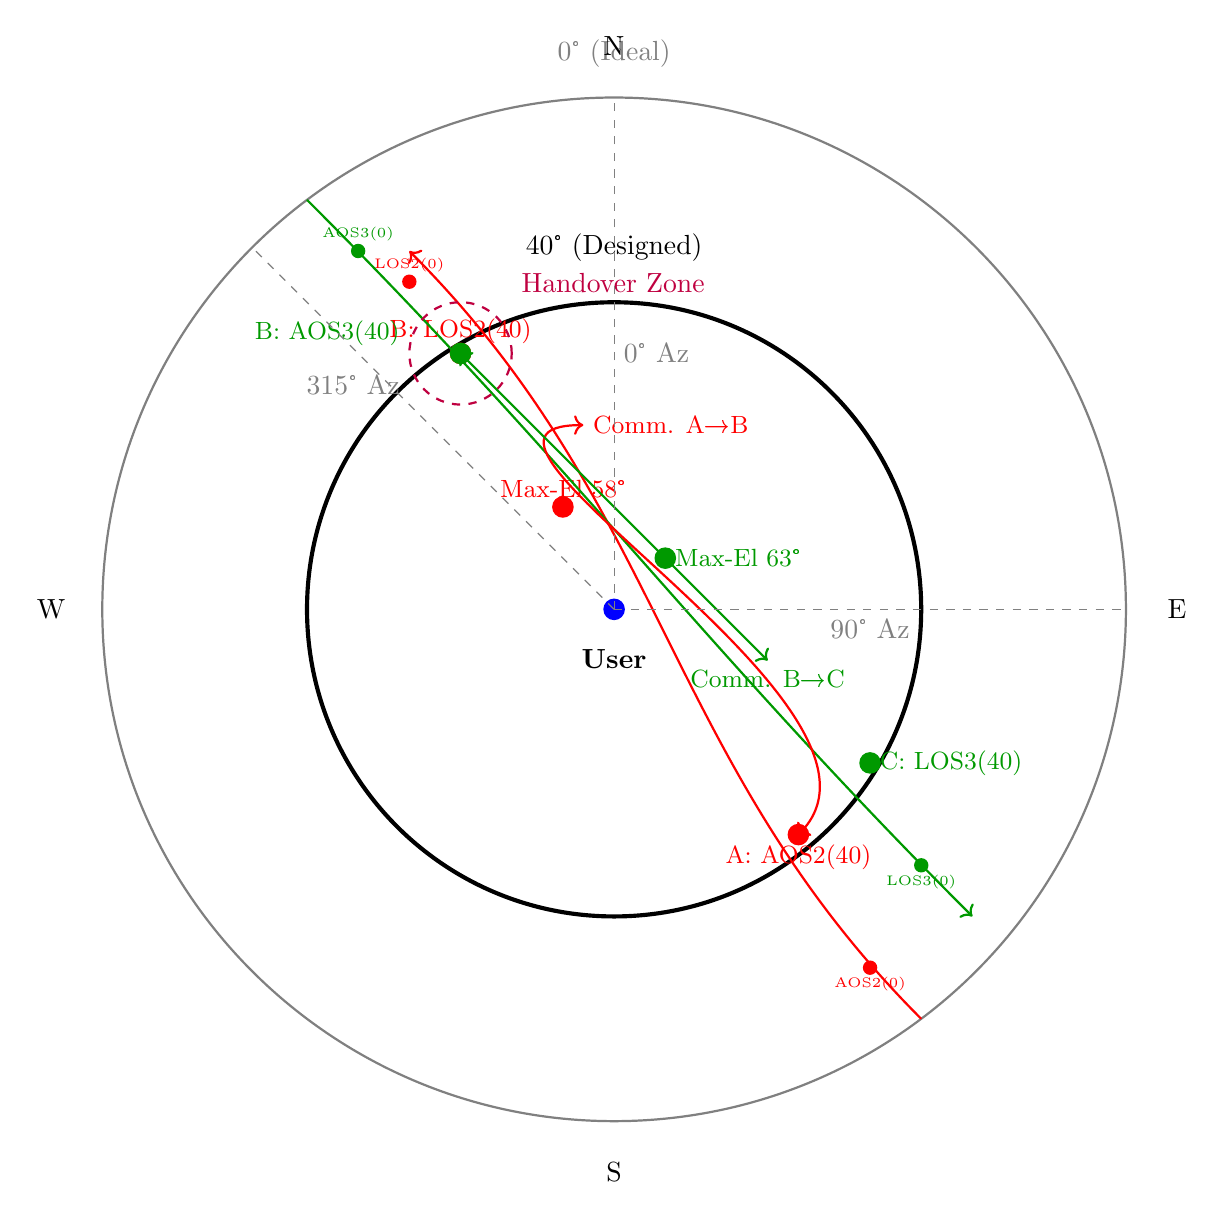
\begin{tikzpicture}[scale=1.3]
    % User at center
    \fill[blue] (0,0) circle (3pt);
    \node[below] at (0,-0.3) {\textbf{User}};

    % Horizon circles
    % Ideal horizon (0°)
    \draw[thick,gray] (0,0) circle (5cm);
    \node[gray,above] at (0,5.2) {0° (Ideal)};

    % Designed horizon (40°)
    \draw[thick,black,line width=1.5pt] (0,0) circle (3cm);
    \node[black,above] at (0,3.3) {40° (Designed)};

    % Compass directions
    \node at (0,5.5) {N};
    \node at (0,-5.5) {S};
    \node at (5.5,0) {E};
    \node at (-5.5,0) {W};

    % Orbit 2 (passes from SE to NW)
    \draw[thick,red,->] (3,-4) to[out=135,in=-45] (-2,3.5);

    % Orbit 2 key points
    \coordinate (aos2_0) at (2.5,-3.5);
    \fill[red] (aos2_0) circle (2pt);
    \node[below,red] at (aos2_0) {\tiny AOS2(0)};

    \coordinate (aos2_40) at (1.8,-2.2);
    \fill[red] (aos2_40) circle (3pt);
    \node[below,red] at (aos2_40) {\small A: AOS2(40)};

    \coordinate (maxel2) at (-0.5,1);
    \fill[red] (maxel2) circle (3pt);
    \node[above,red] at (maxel2) {\small Max-El 58°};

    \coordinate (los2_40) at (-1.5,2.5);
    \fill[red] (los2_40) circle (3pt);
    \node[above,red] at (los2_40) {\small B: LOS2(40)};

    \coordinate (los2_0) at (-2,3.2);
    \fill[red] (los2_0) circle (2pt);
    \node[above,red] at (los2_0) {\tiny LOS2(0)};

    % Orbit 3 (passes from NW to SE)
    \draw[thick,green!60!black,->] (-3,4) to[out=-45,in=135] (3.5,-3);

    % Orbit 3 key points
    \coordinate (aos3_0) at (-2.5,3.5);
    \fill[green!60!black] (aos3_0) circle (2pt);
    \node[above,green!60!black] at (aos3_0) {\tiny AOS3(0)};

    \coordinate (aos3_40) at (-1.5,2.5);
    \fill[green!60!black] (aos3_40) circle (3pt);
    \node[left,green!60!black] at (-2,2.7) {\small B: AOS3(40)};

    \coordinate (maxel3) at (0.5,0.5);
    \fill[green!60!black] (maxel3) circle (3pt);
    \node[right,green!60!black] at (maxel3) {\small Max-El 63°};

    \coordinate (los3_40) at (2.5,- 1.5);
    \fill[green!60!black] (los3_40) circle (3pt);
    \node[right,green!60!black] at (los3_40) {\small C: LOS3(40)};

    \coordinate (los3_0) at (3,-2.5);
    \fill[green!60!black] (los3_0) circle (2pt);
    \node[below,green!60!black] at (los3_0) {\tiny LOS3(0)};

    % Handover zone highlight
    \draw[thick,purple,dashed] (los2_40) circle (0.5cm);
    \node[purple,above right] at (-1,3) {Handover Zone};

    % Communication windows
    \draw[thick,red,<->] (aos2_40) to[out=45,in=180] (-0.3,1.8);
    \node[red,right] at (-0.3,1.8) {\small Comm. A→B};

    \draw[thick,green!60!black,<->] (aos3_40) to[out=-45,in=135] (1.5,-0.5);
    \node[green!60!black,below] at (1.5,-0.5) {\small Comm. B→C};

    % Azimuth angles (selected)
    \draw[dashed,gray] (0,0) -- (5,0);
    \node[gray,below] at (2.5,0) {90° Az};

    \draw[dashed,gray] (0,0) -- (0,5);
    \node[gray,right] at (0,2.5) {0° Az};

    \draw[dashed,gray] (0,0) -- (-3.5,3.5);
    \node[gray,above left] at (-2,2) {315° Az};

\end{tikzpicture}
\end{center}

\textbf{Key Events and Coordinates (from Table 5.5):}

\textbf{Orbit2 (red):}
\begin{itemize}
    \item AOS2(0): [155°, 0°] - enters ideal horizon, not locked
    \item \textbf{Point A - AOS2(40): [220°, 40°]} - locked, comm starts, range = 809.5 km
    \item Max-El: [310°, 58°] - closest approach, range = 641.4 km
    \item \textbf{Point B - LOS2(40): [345°, 40°]} - unlocked, comm ends, range = 809.5 km
    \item LOS2(0): [30°, 0°] - leaves ideal horizon
\end{itemize}

\textbf{Orbit3 (green):}
\begin{itemize}
    \item AOS3(0): [315°, 0°] - enters ideal horizon, not locked
    \item \textbf{Point B - AOS3(40): [345°, 40°]} - locked, comm starts, range = 809.5 km
    \item Max-El: [30°, 63°] - closest approach, range = 611.2 km
    \item \textbf{Point C - LOS3(40): [85°, 40°]} - unlocked, comm ends, range = 809.5 km
    \item LOS3(0): [125°, 0°] - leaves ideal horizon
\end{itemize}

\textbf{Handover at Point B:}
\begin{itemize}
    \item Sat2 at 39° elevation: 827.9 km from user (ready to handover)
    \item Sat3 at 41° elevation: 800.6 km from user (ready to takeover)
    \item Distance between satellites: ≈ 40 km (can communicate via ISL)
    \item User maintains continuous communication: A → B → C
\end{itemize}

\newpage

\section*{Summary of Key Geometric Concepts}

\subsection*{1. Coverage Area}
\begin{itemize}
    \item Circular footprint on Earth's surface
    \item Determined by altitude $H$ and elevation angle $\varepsilon_0$
    \item Larger at higher altitudes and lower elevations
    \item Typical LEO coverage: 1.69\% to 7.95\% of Earth
\end{itemize}

\subsection*{2. Coverage Belt}
\begin{itemize}
    \item Strip of Earth swept during one orbit
    \item Width = $2d_{max}$ where $d_{max} = R_E\sqrt{((H+R_E)/R_E)^2 - 1}$
    \item Range: 3857 to 8178 km for typical LEO altitudes
    \item Moves westward as Earth rotates eastward
\end{itemize}

\subsection*{3. Global Coverage}
\begin{itemize}
    \item Requires constellation of multiple satellites
    \item Coverage areas overlap by 2-5°
    \item Satellites intercommunicate via ISL
    \item Handover ensures continuous service
\end{itemize}

\subsection*{4. Handover Process}
\begin{itemize}
    \item Occurs in overlap zones
    \item LOS of one satellite coincides with AOS of another
    \item Satellites coordinate via ISL
    \item Seamless for user (no service interruption)
\end{itemize}

\end{document}
